\documentclass[journal,12pt,twocolumn]{IEEEtran}
%
\usepackage{setspace}
\usepackage{multicol}
\usepackage{gensymb}
\usepackage{enumerate}
\usepackage{xcolor}
\usepackage{caption}
%\usepackage{subcaption}
%\doublespacing
\singlespacing
%\usepackage{epstopdf}
%\usepackage{graphicx}
%\usepackage{amssymb}
%\usepackage{relsize}
\usepackage[cmex10]{amsmath}
\usepackage{mathtools}
%\usepackage{amsthm}
%\interdisplaylinepenalty=2500
%\savesymbol{iint}
%\usepackage{txfonts}
%\restoresymbol{TXF}{iint}
%\usepackage{wasysym}
\usepackage{amsthm}
\usepackage{mathrsfs}
\usepackage{txfonts}
\usepackage{stfloats}
\usepackage{cite}
\usepackage{cases}
\usepackage{subfig}
%\usepackage{xtab}
\usepackage{longtable}
\usepackage{multirow}
%\usepackage{algorithm}
%\usepackage{algpseudocode}
%\usepackage{enumitem}
\usepackage{mathtools}
\usepackage{iithtlc}
%\usepackage[framemethod=tikz]{mdframed}
\usepackage{listings}
\usepackage{amsmath}
\usepackage{polynomial}

%\usepackage{stmaryrd}


%\usepackage{wasysym}
%\newcounter{MYtempeqncnt}
\DeclareMathOperator*{\Res}{Res}
%\renewcommand{\baselinestretch}{2}
\renewcommand\thesection{\arabic{section}}
\renewcommand\thesubsection{\thesection.\arabic{subsection}}
\renewcommand\thesubsubsection{\thesubsection.\arabic{subsubsection}}

\renewcommand\thesectiondis{\arabic{section}}
\renewcommand\thesubsectiondis{\thesectiondis.\arabic{subsection}}
\renewcommand\thesubsubsectiondis{\thesubsectiondis.\arabic{subsubsection}}

% correct bad hyphenation here
\hyphenation{op-tical net-works semi-conduc-tor}

\lstset{
language=Python,
frame=single, 
breaklines=true
}

%\lstset{
	%%basicstyle=\small\ttfamily\bfseries,
	%%numberstyle=\small\ttfamily,
	%language=python,
	%backgroundcolor=\color{white},
	%%frame=single,
	%%keywordstyle=\bfseries,
	%%breaklines=true,
	%%showstringspaces=false,
	%%xleftmargin=-10mm,
	%%aboveskip=-1mm,
	%%belowskip=0mm
%}

%\surroundwithmdframed[width=\columnwidth]{lstlisting}


\begin{document}
%

\theoremstyle{definition}
\newtheorem{theorem}{Theorem}[section]
%\newtheorem{problem}{Problem}[section]
\newtheorem{problem}{Problem}
\newtheorem{proposition}{Proposition}
%\newtheorem{proposition}{Proposition}[section]
\newtheorem{lemma}{Lemma}[section]
\newtheorem{corollary}[theorem]{Corollary}
\newtheorem{example}{Example}[section]
%\newtheorem{definition}{Definition}[section]
\newtheorem{definition}{Definition}
%\newtheorem{definition}{Definition}
%\newtheorem{algorithm}{Algorithm}[section]
%\newtheorem{cor}{Corollary}
\newcommand{\BEQA}{\begin{eqnarray}}
\newcommand{\EEQA}{\end{eqnarray}}
\newcommand{\define}{\stackrel{\triangle}{=}}

\bibliographystyle{IEEEtran}
%\bibliographystyle{ieeetr}

\providecommand{\nCr}[2]{\,^{#1}C_{#2}} % nCr
\providecommand{\nPr}[2]{\,^{#1}P_{#2}} % nPr
\providecommand{\mbf}{\mathbf}
\providecommand{\pr}[1]{\ensuremath{\Pr\left(#1\right)}}
\providecommand{\qfunc}[1]{\ensuremath{Q\left(#1\right)}}
\providecommand{\sbrak}[1]{\ensuremath{{}\left[#1\right]}}
\providecommand{\lsbrak}[1]{\ensuremath{{}\left[#1\right.}}
\providecommand{\rsbrak}[1]{\ensuremath{{}\left.#1\right]}}
\providecommand{\brak}[1]{\ensuremath{\left(#1\right)}}
\providecommand{\lbrak}[1]{\ensuremath{\left(#1\right.}}
\providecommand{\rbrak}[1]{\ensuremath{\left.#1\right)}}
\providecommand{\cbrak}[1]{\ensuremath{\left\{#1\right\}}}
\providecommand{\lcbrak}[1]{\ensuremath{\left\{#1\right.}}
\providecommand{\rcbrak}[1]{\ensuremath{\left.#1\right\}}}
\theoremstyle{remark}
\newtheorem{rem}{Remark}
\newcommand{\sgn}{\mathop{\mathrm{sgn}}}
\providecommand{\abs}[1]{\left\vert#1\right\vert}
\providecommand{\res}[1]{\Res\displaylimits_{#1}} 
\providecommand{\norm}[1]{\lVert#1\rVert}
\providecommand{\mtx}[1]{\mathbf{#1}}
\providecommand{\mean}[1]{E\left[ #1 \right]}
\providecommand{\fourier}{\overset{\mathcal{F}}{ \rightleftharpoons}}
%\providecommand{\hilbert}{\overset{\mathcal{H}}{ \rightleftharpoons}}
\providecommand{\system}{\overset{\mathcal{H}}{ \longleftrightarrow}}
	%\newcommand{\solution}[2]{\textbf{Solution:}{#1}}
\newcommand{\solution}{\noindent \textbf{Solution: }}
\providecommand{\dec}[2]{\ensuremath{\overset{#1}{\underset{#2}{\gtrless}}}}
%\numberwithin{equation}{section}
\numberwithin{equation}{problem}
%\numberwithin{problem}{subsection}
%\numberwithin{definition}{subsection}
\makeatletter
\@addtoreset{figure}{problem}
\makeatother

\let\StandardTheFigure\thefigure
%\renewcommand{\thefigure}{\theproblem.\arabic{figure}}
\renewcommand{\thefigure}{\theproblem}


%\numberwithin{figure}{subsection}

\def\putbox#1#2#3{\makebox[0in][l]{\makebox[#1][l]{}\raisebox{\baselineskip}[0in][0in]{\raisebox{#2}[0in][0in]{#3}}}}
     \def\rightbox#1{\makebox[0in][r]{#1}}
     \def\centbox#1{\makebox[0in]{#1}}
     \def\topbox#1{\raisebox{-\baselineskip}[0in][0in]{#1}}
     \def\midbox#1{\raisebox{-0.5\baselineskip}[0in][0in]{#1}}

\vspace{3cm}

\title{ 
\logo{
Differentiation
}
%	\logo{python for Math Computing }
}
%\title{
%	\logo{Matrix Analysis through python}{\begin{center}\includegraphics[scale=.24]{tlc}\end{center}}{}{HAMDSP}
%}


% paper title
% can use linebreaks \\ within to get better formatting as desired
%\title{Matrix Analysis through python}
%
%
% author names and IEEE memberships
% note positions of commas and nonbreaking spaces ( ~ ) LaTeX will not break
% a structure at a ~ so this keeps an author's name from being broken across
% two lines.
% use \thanks{} to gain access to the first footnote area
% a separate \thanks must be used for each paragraph as LaTeX2e's \thanks
% was not built to handle multiple paragraphs
%

\author{P.~N.~V.~S.~S.~K.~ HAVISH$^{*}$, S.~S.~Ashish$^{*}$, J.~Balasubramaniam$^{\dagger}$ and G V V Sharma$^{*}$ %<-this  stops a space
\thanks{$\dagger$ The author is with the Department of Mathematics, IIT Hyderabad.  *The authors are with the Department
of Electrical Engineering, IIT, Hyderabad
502285 India e-mail: \{ee16btech11023,ee16btech11043,jbala,gadepall\}@iith.ac.in. All material in the manuscript is released under GNU GPL.  Free to use for all.}% <-this % stops a space
%\thanks{J. Doe and J. Doe are with Anonymous University.}% <-this % stops a space
%\thanks{Manuscript received April 19, 2005; revised January 11, 2007.}}
}
% note the % following the last \IEEEmembership and also \thanks - 
% these prevent an unwanted space from occurring between the last author name
% and the end of the author line. i.e., if you had this:
% 
% \author{....lastname \thanks{...} \thanks{...} }
%                     ^------------^------------^----Do not want these spaces!
%
% a space would be appended to the last name and could cause every name on that
% line to be shifted left slightly. This is one of those "LaTeX things". For
% instance, "\textbf{A} \textbf{B}" will typeset as "A B" not "AB". To get
% "AB" then you have to do: "\textbf{A}\textbf{B}"
% \thanks is no different in this regard, so shield the last } of each \thanks
% that ends a line with a % and do not let a space in before the next \thanks.
% Spaces after \IEEEmembership other than the last one are OK (and needed) as
% you are supposed to have spaces between the names. For what it is worth,
% this is a minor point as most people would not even notice if the said evil
% space somehow managed to creep in.



% The paper headers
%\markboth{Journal of \LaTeX\ Class Files,~Vol.~6, No.~1, January~2007}%
%{Shell \MakeLowercase{\textit{et al.}}: Bare Demo of IEEEtran.cls for Journals}
% The only time the second header will appear is for the odd numbered pages
% after the title page when using the twoside option.
% 
% *** Note that you probably will NOT want to include the author's ***
% *** name in the headers of peer review papers.                   ***
% You can use \ifCLASSOPTIONpeerreview for conditional compilation here if
% you desire.




% If you want to put a publisher's ID mark on the page you can do it like
% this:
%\IEEEpubid{0000--0000/00\$00.00~\copyright~2007 IEEE}
% Remember, if you use this you must call \IEEEpubidadjcol in the second
% column for its text to clear the IEEEpubid mark.



% make the title area
\maketitle

%\newpage

%\tableofcontents


%\begin{abstract}
%%\boldmath
%In this letter, an algorithm for evaluating the exact analytical bit error rate  (BER)  for the piecewise linear (PL) combiner for  multiple relays is presented. Previous results were available only for upto three relays. The algorithm is unique in the sense that  the actual mathematical expressions, that are prohibitively large, need not be explicitly obtained. The diversity gain due to multiple relays is shown through plots of the analytical BER, well supported by simulations. 
%
%\end{abstract}
% IEEEtran.cls defaults to using nonbold math in the Abstract.
% This preserves the distinction between vectors and scalars. However,
% if the journal you are submitting to favors bold math in the abstract,
% then you can use LaTeX's standard command \boldmath at the very start
% of the abstract to achieve this. Many IEEE journals frown on math
% in the abstract anyway.

% Note that keywords are not normally used for peerreview papers.
%\begin{IEEEkeywords}
%Cooperative diversity, decode and forward, piecewise linear
%\end{IEEEkeywords}



% For peer review papers, you can put extra information on the cover
% page as needed:
% \ifCLASSOPTIONpeerreview
% \begin{center} \bfseries EDICS Category: 3-BBND \end{center}
% \fi
%
% For peerreview papers, this IEEEtran command inserts a page break and
% creates the second title. It will be ignored for other modes.
\IEEEpeerreviewmaketitle

\bigskip

\begin{abstract}
This manual discusses problems related to differentiation through examples.  Python scripts are provided to supplement the theory.
\end{abstract}
%
\begin{definition}
\label{def:derivative}
Suppose $f$ is  a real function and c is a point in its domain.The derivative of f at c is defined by 
%For every $\epsilon > 0$, there exists a $\delta > 0$ such that 
\begin{equation}
\lim_{h \to 0} {\frac {f(c+h)-f(c)}{h}}
\end{equation}
provided this limit exists.
In general 
\begin{equation}
f'(x)=\lim_{h \to 0} {\frac {f(x+h)-f(x)}{h}}
\end{equation}
\end{definition}
%\section{Limit}
\begin{problem}
Find the derivative of the function $f(x)=\sqrt{2x-1}$ from the definition
\end{problem}
%
\begin{proof}

Using Definition \ref{def:derivative},
  
\begin{align}
f'(x)=\lim_{h \to 0} {\frac{\sqrt{2(x+h)-1}-\sqrt{2x-1}}{h}}\\
     =\lim_{h \to 0} {\frac{2(x+h)-1-2x+1}{h(\sqrt{2(x+h)-1}+\sqrt{2x-1})}} \\
=\lim_{h \to 0} {\frac{2h}{h(\sqrt{2(x+h)-1}+\sqrt{2x-1})}}
\end{align}
\begin{align}
f'(x)=\frac{1}{\sqrt{2x-1}}
\end{align}
The following code plots the derivative of $f(x)$. Fig. \ref{fig:1} verifies that the derivative is indeed $\frac{1}{\sqrt{2x-1}}$.
\lstinputlisting{./codes/1.py}
%
\begin{figure}[!ht]
\begin{center}
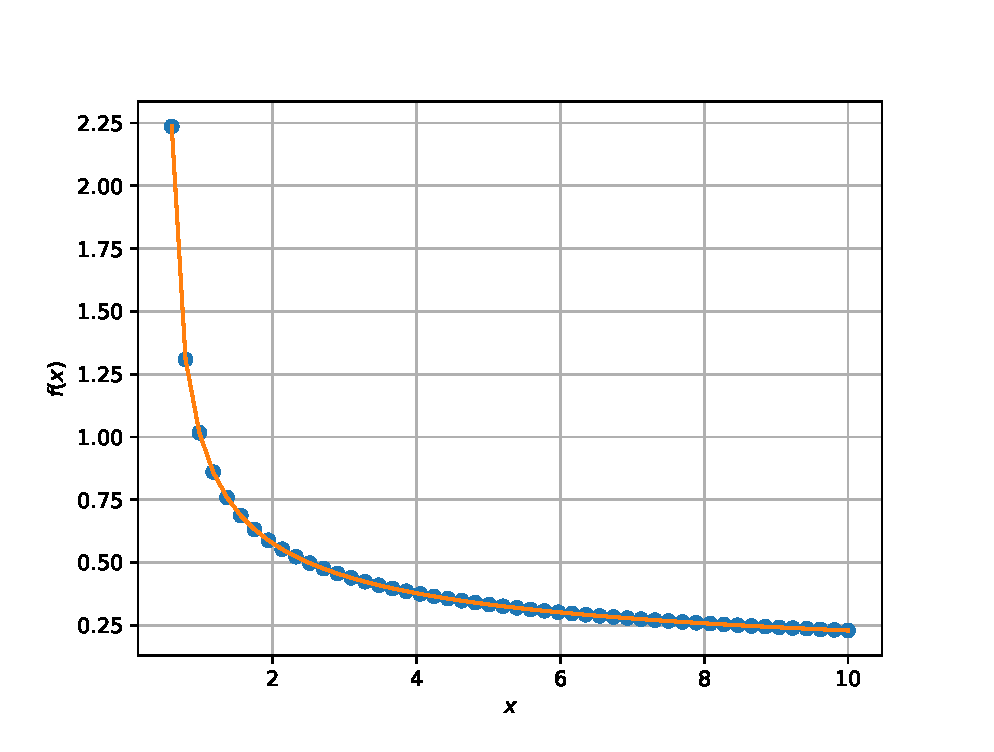
\includegraphics[width=\columnwidth]{./figs/1.eps}
\end{center}
\captionof{figure}{}

\label{fig:1}	
\end{figure}
\end{proof}
%
%\begin{problem}
%
%Verify that
%\begin{equation}
%\abs{\sin x} \leq \abs{x}
%\end{equation}
%\end{problem}
%\solution The following code yields Fig. \ref{fig:2}.
%\lstinputlisting{./codes/2.py}
%%
%\begin{figure}[!ht]
%\begin{center}
%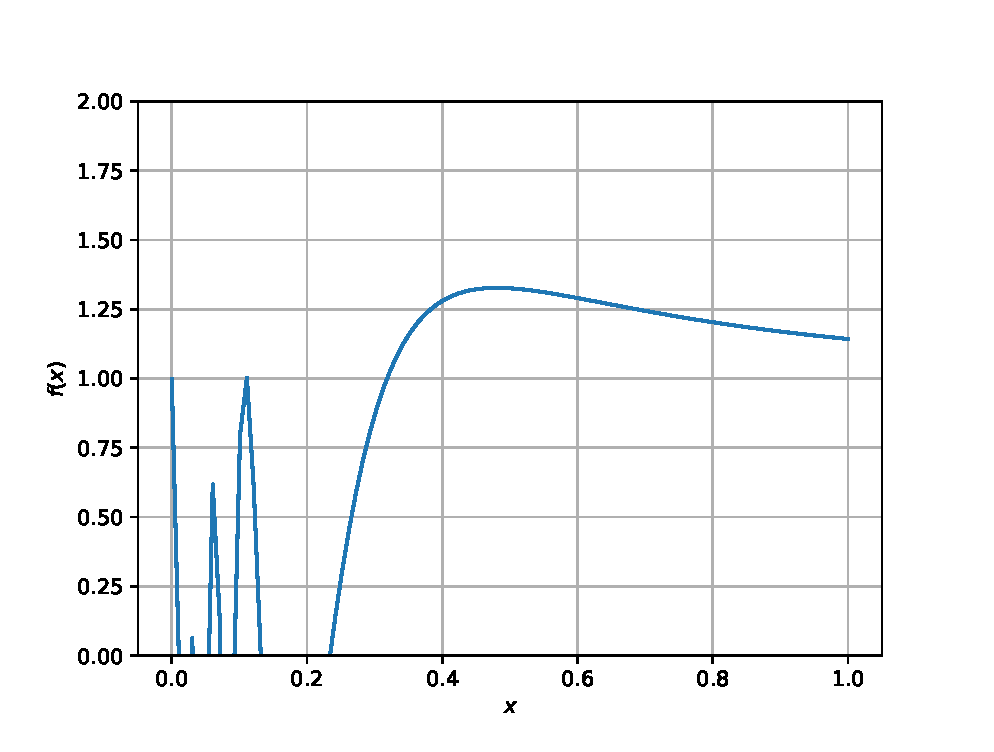
\includegraphics[width=\columnwidth]{./figs/2.eps}
%\end{center}
%\captionof{figure}{$\abs{\sin x} \le \abs{x}$}
%\label{fig:2}	
%\end{figure}
%
\begin{problem}
Let 
\begin{equation}
f(x)=
 \begin{cases} 
      x^2\sin\brak{\frac{1}{x}} & x \neq 0 \\
      0 & x=0  
   \end{cases}
\end{equation}
\begin{itemize}
\item Is $f$ differentiable at x=0
\item Is $f'$ continuous at x=0
\end{itemize}
\end{problem}
%%
\begin{proof}
From Definition \ref{def:derivative},

\begin{align}
f'(0)=\lim_{h \to 0} {\frac {f(0+h)-f(0)}{h}}=\lim_{h \to 0} {\frac{h^2\sin\brak{\frac{1}{h}}-0}{h}}=0
\end{align}
From eq(2.2) we can conclude that $f(x)$ is differentiable at x=0.\\
Now,
\begin{equation}
f'(x)=
 \begin{cases} 
      2x\sin\brak{\frac{1}{x}}-\cos\brak{\frac{1}{x}} & x \neq 0\\
      0 & x=0  
   \end{cases}
\end{equation}
which is  not continuous as the $\cos\brak{\frac{1}{x}}$ oscillates between -1 and 1 as $x\to 0$ whereas $f(x)=0$ at $x=0$.\\
Thus $f'(x)$ is not continuous at x=0.\\
Hence $f(x)$ is not continuously differentiable.
The following code plots $f(x)$ as $x \to 0$. Fig. \ref{fig:2} verifying that $f'(x)$ is indeed discontinuous at $x=0$.
\lstinputlisting{./codes/2.py}
%
\begin{figure}[!ht]
\begin{center}
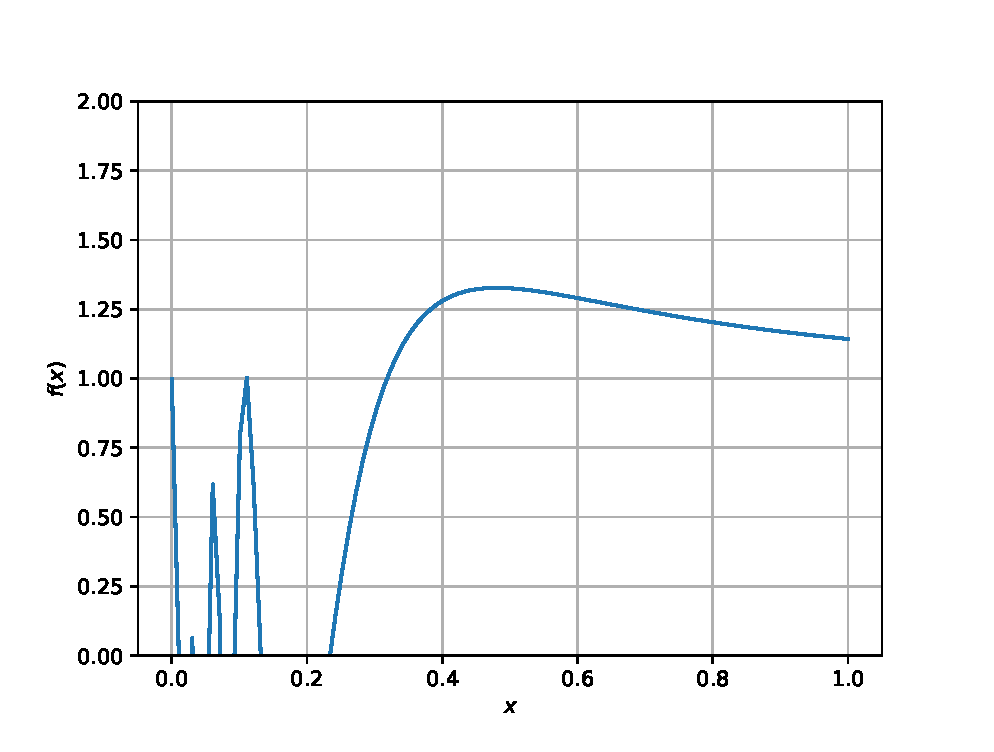
\includegraphics[width=\columnwidth]{./figs/2.eps}
\end{center}
\captionof{figure}{}
\label{fig:2}	
\end{figure}
\end{proof}



%\begin{problem}
%Investigate the continuity of the following function at $x=x_0$
%%
%\begin{equation}
%f(x)=
% \begin{cases} 
%      \sin(\pi x) & 0<x < 1 \\
%      \ln (x) & 1< x< 2  
%   \end{cases},x_0=1
%\end{equation}
%\end{problem}
%%
%%\begin{proof}
%\solution The following code plots $f(x)$ and  
%Fig. \ref{fig:4} indicates that $f(x)$ is indeed continuous at $x_0=1$.
%
%\lstinputlisting{./codes/4.py}
%%%
%\begin{figure}[!ht]
%\begin{center}
%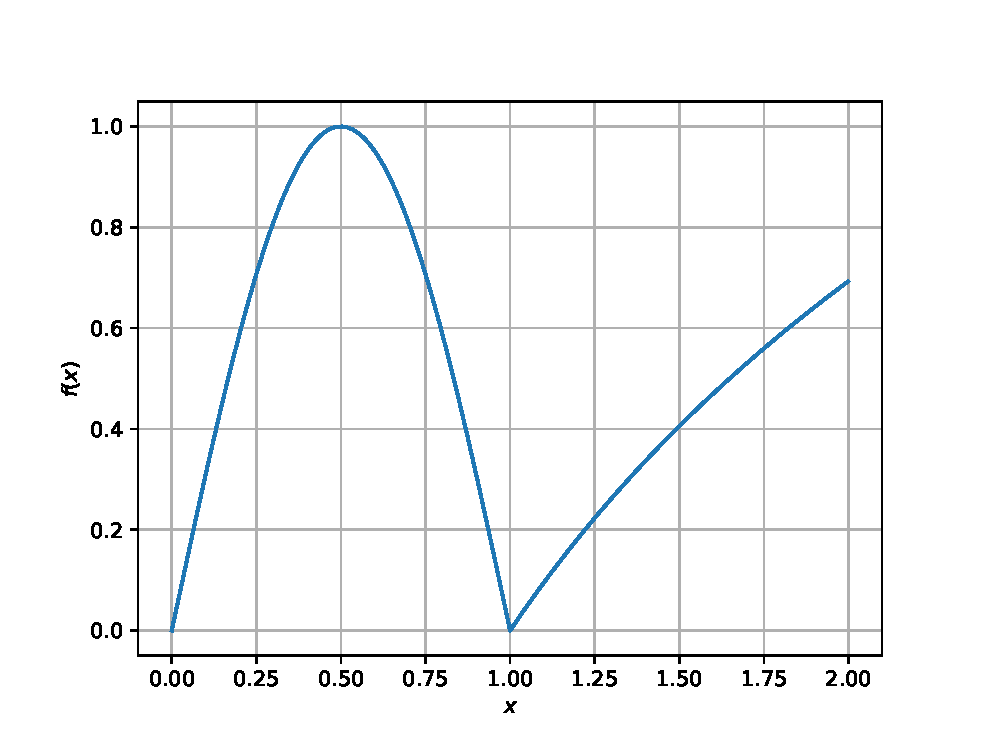
\includegraphics[width=\columnwidth]{./figs/4.eps}
%\end{center}
%\captionof{figure}{}
%\label{fig:4}	
%\end{figure} 
%
%Consider the left limit at $x_0=1$. 
%%$f(x)=\sin \pi x$ as $x \to 1$ from left.
%So, 
%\begin{equation}
%\lim_{x \to 1^-} f(x)=\lim_{x\to 1^{-}} \sin(\pi x)=\sin(\pi)=0.
%\end{equation}
%%
%Similarly, 
%%$f(x)=\ln(x)$ as $x \to 1$ from right. 
%\begin{equation}
%\lim_{x \to 1^+} f(x)=\lim_{x \to 1^{+}} \ln(x)=\ln(1)=0.
%\end{equation}
%From Definition \ref{def:continutiy},
%%Clearly the left limit and right limit of $f(x)$ at $x_0=1$ are equal and $0$. 
%$f(x)$ is continuous at $x_0=1$.
%%\end{proof}

\begin{proposition}
\label{prop: L'Hospital's Rule}
(L'Hospital's Rule) \\ If $f$ and $g$ are two differentiable functions, and 
\begin{align}
\lim_{x \to a}{\frac{f(x)}{g(x)}}=\frac{0}{0} \\
  OR  \hspace{0.75cm}\\ 
\lim_{x \to a}{\frac{f(x)}{g(x)}}=\frac{\infty}{\infty}
\end{align}
in these cases we have 
\begin{align}
\lim_{x \to a}{\frac{f(x)}{g(x)}}=\lim_{x \to a}{\frac{f^n(x)}{g^n(x)}}
\end{align}
as long as the indeterminate form holds and the derivatives exist.
%\begin{itemize}
%\item $f+g$
%\item $f-g$
%\item $fg$
%\item $\frac{f}{g}$
%\end{itemize}
%are also continuous wherever they are defined. Note that the similar properties hold for limits at any point $a$.
\end{proposition}
\begin{problem}
Use L'Hospital's Rule to evaluate $\lim_{x \to 0}{\frac{e^{2x}-1}{x}}$.
\end{problem}
\solution  
\begin{align}
\lim_{x \to 0}{\frac{e^{2x}-1}{x}}=\frac{0}{0}
\end{align}
By using Proposition \ref{prop: L'Hospital's Rule}
\begin{align}
\lim_{x \to 0}{\frac{e^{2x}-1}{x}}=\lim_{x \to 0}{\frac{\frac{d(e^{2x}-1)}{dx}}{\frac{x}{dx}}}=
   \lim_{x \to 0}{\frac{2e^{2x}}{1}}=2
\end{align}

\begin{problem}
Use L'Hospital's Rule to evaluate $\lim_{x \to 0}{\brak{cos\brak{x}}^{\frac{1}{x^2}}}$.
\end{problem}
\solution  
\begin{align}
f(x)=\brak{cos\brak{x}}^{\frac{1}{x^2}}
\implies
\lim_{x \to 0}{f(x)}=1^\infty
\end{align}
\begin{align}
g(x)=\log\brak{f(x)}=\frac{\log\brak{cosx}}{x^2}
\end{align}
By using Proposition \ref{prop: L'Hospital's Rule}
\begin{align}
\lim_{x \to 0}{g(x)}=\lim_{x \to 0}{\frac{\log\brak{cosx}}{x^2}}=\lim_{x \to 0}{\frac{-tanx}{2x}}
\\=\lim_{x \to 0}{\frac{-\brak{secx}^2}{2}}
\implies\lim_{x \to 0}{f(x)}=e^{-0.5}
\end{align}
$\therefore$ required limit is $e^{-0.5}$.

%\lstinputlisting{./codes/5.py}
%%%
%\begin{figure}[!ht]
%\begin{center}
%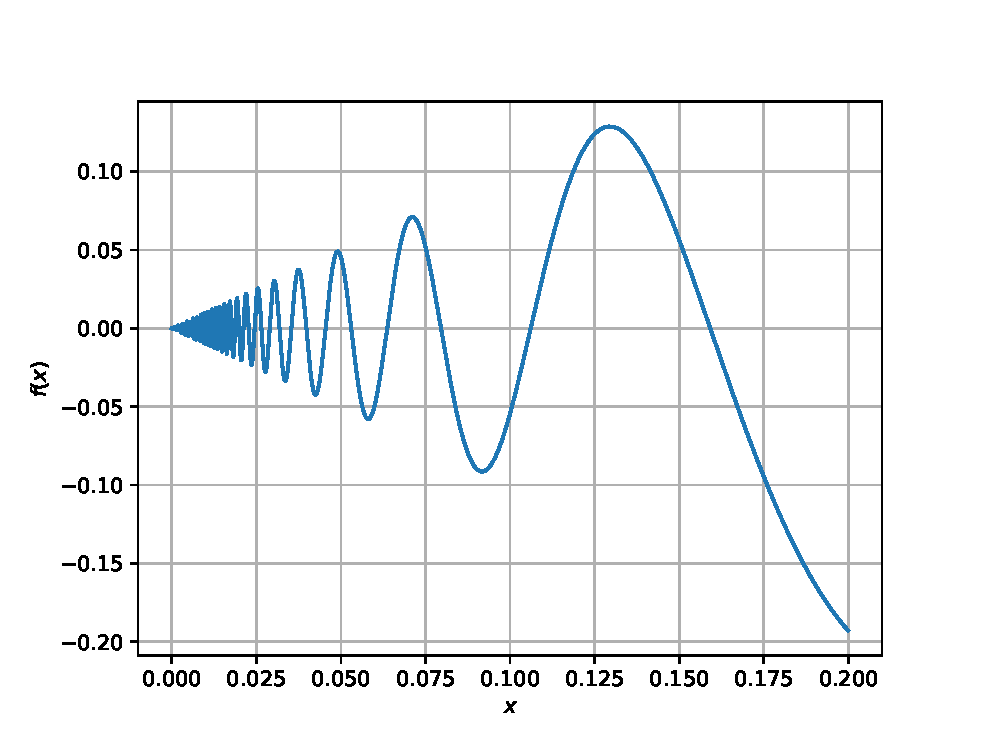
\includegraphics[width=\columnwidth]{./figs/5.eps}
%\end{center}
%\captionof{figure}{}
%\label{fig:5}	
%\end{figure} 
%%
%Rearranging the given function as
%\begin{equation}
%f(x)=\frac{x \sin\brak{\frac{1}{x}}}{\frac{\sin(x)}{x}}
%\end{equation}
%Let 
%\begin{equation}
%g(x)=x \sin\brak{\frac{1}{x}}, h(x)=\frac{\sin(x)}{x}
%\end{equation}
%%
%By proposition \ref{prop: Properties of continuous functions}, 
%\begin{equation}
%\label{eq:lim_ratio}
%\lim_{x \to 0}f(x)= \frac{\lim_{x\to 0}g(x)}{\lim_{x\to 0}h(x)}.
%\end{equation}
%%
%$\because \lim_{x \to 0} g(x) = 0$ and  $\lim_{x \to 0} h(x) = 1$, from \eqref{eq:lim_ratio},
%
%$\lim_{x\to 0}f(x)=\frac{0}{1}=0$. 
%%
\begin{problem}
Use L'Hospital's Rule to evaluate $\lim_{x \to \infty}{(x-\sqrt{x+x^2})}$.
\end{problem}
\solution On rationalising $f(x)$ 
\begin{align}
\lim_{x \to \infty}{(x-\sqrt{x+x^2})}=\lim_{x \to \infty}{\frac{(x-\sqrt{x+x^2})(x+\sqrt{x+x^2})}{(x+\sqrt{x+x^2})}}\\
=\lim_{x \to \infty}{\frac{-x}{(x+\sqrt{x+x^2})}}
\end{align}
Now,\\\\
$lim_{x \to \infty}{\frac{-x}{(x+\sqrt{x+x^2})}}$is of the form $\frac{\infty}{\infty}$
By using Proposition \ref{prop: L'Hospital's Rule}
\begin{align}
\lim_{x \to \infty}{\frac{-x}{(x+\sqrt{x+x^2})}}=\lim_{x \to \infty}{\frac{\frac{d(-x)}{dx}}{\frac{d(x+\sqrt{x+x^2})}{dx}}}\\
=\lim_{x \to \infty}{\frac{-1}{1+\frac{1+2x}{2\sqrt{x+x^2}}}}=0
\end{align}
%%\lstinputlisting{./codes/6.py}
%%%%
%%\begin{figure}[!ht]
%%\begin{center}
%%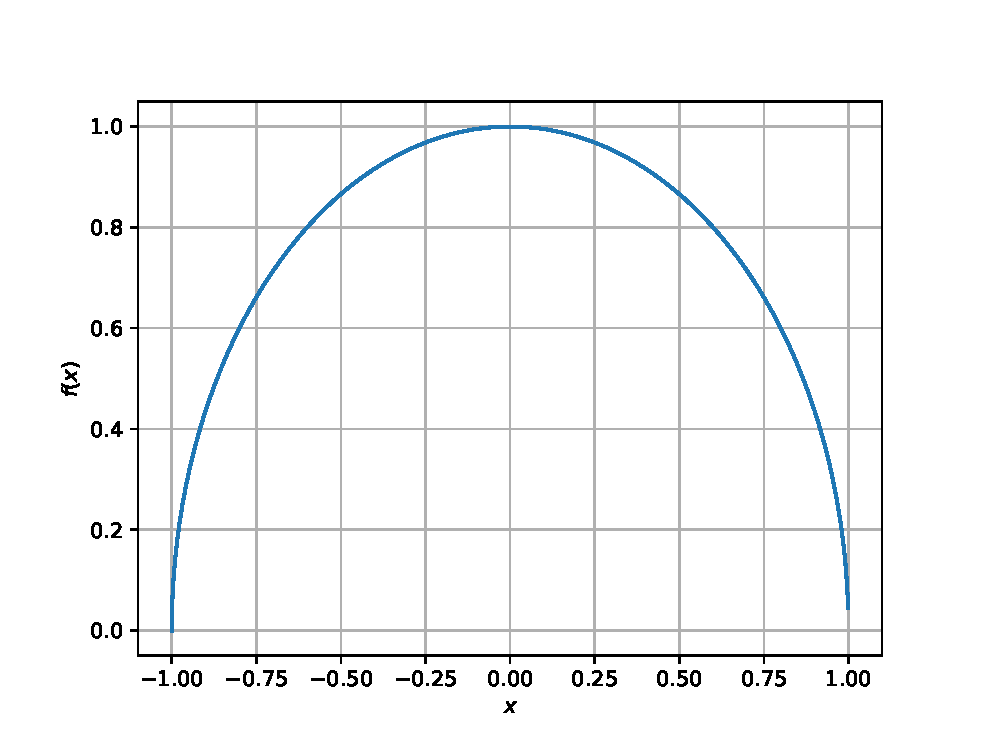
\includegraphics[width=\columnwidth]{./figs/6.eps}
%%\end{center}
%%\captionof{figure}{$f(x)=\sqrt{1-x^2}$}
%%\label{fig:6}	
%%\end{figure} 
%%
%%The function $f(x)$ is continuous for all $x$ for which it is defined. $f(x)$ is defined for $x$ such that
%%\begin{align}
%%1-x^2 \ge 0 \implies \abs{x} \le 1
%%\end{align}
%%%Here $f(x)=\sqrt{1-x^2}$ is defined only for values of $x$ for which $1-x^2 \ge 0$.
%%%\\
%%%$\implies \abs{x} \le 1$. 
%%%For other values of $x$, the function is not defined. 
%%$\therefore$ the domain of continuity of $f(x)$ is $\abs{x} \le 1$ 
%\begin{proposition}
%\label{prop: Sandwich Principle}
%Let I be an interval having the point $a$ as a limit point. Let $g$, $f$ and $h$ be functions defined on I, except possibly at $a$ itself. Suppose that for every $x$ in I not equal to $a$, we have
%\begin{align}
%g(x) \leq f(x) \leq h(x) 
%\end{align} and also if $\lim_{x \to a} g(x) = \lim_{x \to a} h(x) = L$ then $\lim_{x \to a} f(x) = L$.
%\end{proposition}
%\begin{problem}
%Prove that 
%\begin{equation}
%f(x)= \begin{cases} 
%      x \sin\brak{\frac{1}{x}} & x\neq 0 \\
%      5 & x= 0  
%   \end{cases}
%\end{equation}
%is discontinuous at $x=0$ and redefine $f(x)$ such that it is continuous at $x=0$.
%\end{problem}
%\begin{proof}
%The following code plots $f(x)$ where $f(0)=5$ in the upper half and $f(0)=0$ in the lower half. From upper half of Fig. \ref{fig:7} it is trivial that $f(x)$ is discontinuous at $x=0$ and if $f(0)=0$, it is trivial that it is continuous.
%\lstinputlisting{./codes/7.py}
%%
%\begin{figure}[!ht]
%\begin{center}
%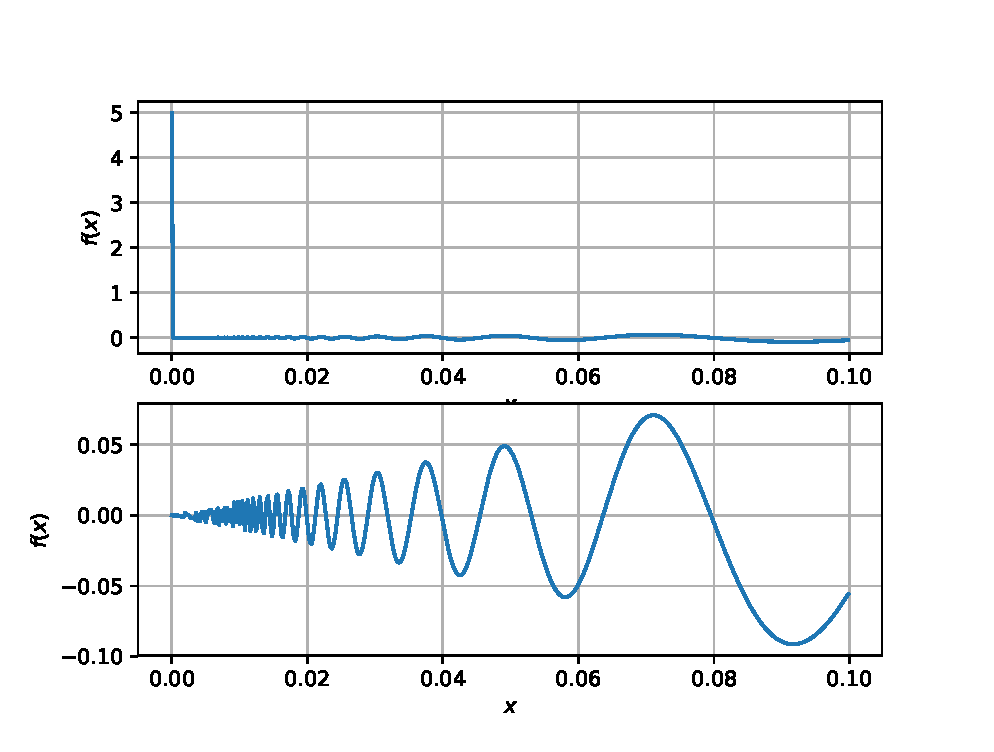
\includegraphics[width=\columnwidth]{./figs/7.eps}
%\end{center}
%\captionof{figure}{}
%\label{fig:7}	
%\end{figure} 
%%
%$\because$
%\begin{align}
%-1\le \sin\brak{\frac{1}{x}} \le 1 \implies -x\leq x\sin\brak{\frac{1}{x}} \leq x, x > 0,
%\end{align} 
%from Proposition \ref{prop: Sandwich Principle}, as $x\to 0+, x\sin \brak{\frac{1}{x}} \to 0$. It can be shown that this is true when
%$x \to 0-$.
%So $\lim_{x \to 0} f(x) = 0$. According to Definition \ref{def:continutiy}, $\lim_{x \to 0} f(x) = f(0)$.
%But $f(0)=5\neq 0$. $\therefore f(x)$ is discontinuous at $x=0$.
%For $f(x)$ to be continuous at $x=0$ define $f(0) = 0$.
%\end{proof}
%
%
%\begin{problem}
%Prove that all polynomials of finite degree over $\mathbb{R}$ are continuous.
%\end{problem}
%\begin{proof}
%Consider a function $f(x)$ such that
%\begin{align}
%f(x)=a_0+a_1x+a_2x^2+......+a_nx^n
%\end{align}
%Clearly $f(x)$ is a linear combination of some real numbers and the powers of $x$.
%So if $g(x)$=$x$ is continuous, then by Proposition \ref{prop: Properties of continuous functions} we can say that $f(x)$ is continuous.
%By definition \ref{def:continutiy} it can be trivially shown that $g(x)$ is continuous. So, $f(x)$ is continuous. 
%\end{proof}
%%
%%\newpage
%\begin{problem}
%Give examples of the following:
%\begin{enumerate}
%\item Function which is continuous at finite number of points.
%\item Function which is nowhere continuous on $\mathbb{R}$.
%\end{enumerate}
%\end{problem}
%\solution
%\begin{enumerate}
%\item \begin{equation}
%f(x)=
% \begin{cases} 
%      (x-2)(x-3) & x\in\mathbb{Q} \\
%      0 & x\in\mathbb{R}-\mathbb{Q} \\ 
%   \end{cases}
%\end{equation}
%which is continuous only at $x=2,x=3$.
%
%\item
%\begin{equation}
%f(x)= \begin{cases} 
%      1 & x\in\mathbb{Q} \\
%      0 & x\in\mathbb{R}-\mathbb{Q} \\ 
%   \end{cases}
%\end{equation}
%
%\end{enumerate}
%
%
%
%\begin{problem}
%Consider two continuous functions $f(x),g(x)$ such that $f(x)=g(x)$ for every rational $x$. Prove that equality holds for all $x$ in $\mathbb{R}$ 
%\end{problem}
%\begin{proof}
%Consider the function 
%\begin{align}
%h(x)=f(x)-g(x),x\in\mathbb{R}
%\end{align} 
%By proposition \ref{prop: Properties of continuous functions}, $h(x)$ is continuous at all real $x$.
%Consider an arbitrary rational number $c$ and its $\delta$ neighborhood. Clearly $h(x)$ is equal to zero at all rational $x$.
%$\because h(x)$ is continuous $\lim_{x \to c} h(x) = h(c) =0$. 
%This implies that $h(x)$ must be zero even in the neighborhood of $c$ which consists of infinite number of irrationals. 
%$\therefore h(x) = 0$ for all $x \in \mathbb{R}$.
%$h(x) = 0\implies f(x)=g(x), x \in \mathbb{R}$.
%\end{proof}
%
%\begin{proposition}
%\label{prop: Location of roots Theorem}
%Consider a function $f:I \to \mathbb{R}$ where $I=[a,b]$. If $f(a)<0<f(b)$ or $f(a)>0>f(b)$, then $\ni c \in$ I such that $f(c)=0$.
%\end{proposition}
%\begin{problem}
%Show that every polynomial of odd degree with real coefficients has atleast one real root.
%\end{problem}
%\begin{proof}
%Consider $f(x)=a_0+a_1x+a_2x^2+......+a_nx^n$, $n$ is odd. Let $g(x)=\frac{f(x)}{x^n}=\frac{a_0}{x^n} + \frac{a_1x}{x^n} + \frac{a_2x^2}{x^n} + ...... +a_n$. Consider the interval $[a,b]$ where $a\ll0,b\gg0$ 
%$g(a) \to 1$ as $a \to -\infty$. Similarly $g(b) \to 1$ as $b \to \infty$. 
%$\because n$ is odd, for negative values of $x$, $x^n <0$ and for positive values of $x$ it is $x^n>0$. But $g(x)=\frac{f(x)}{x^n}=1>0$ in both cases. So $f(x) < 0$ at $x=a$ and $f(x) >0$ at $x=b$. $\therefore$ by proposition \ref{prop: Location of roots Theorem}, $f(x)$ has atleast one root in the interval I. Hence, proved.  
%\end{proof}
%\begin{proposition}
%\label{prop: Intermediate value theorem}
%Consider a function $f:I \to \mathbb{R}$ where $I=[a,b]$. If $f(a)<k<f(b),k\in\mathbb{R}$, then $\ni c\in I$ such that $f(c)=k$.
%\end{proposition}
%\begin{problem}
%Let I=[0,1] and $f(0)=f(1)$ where $f$ is continuous on I. Prove that $\ni c \in[0,\frac{1}{2}]$ such that  $f(c)=f(c+\frac{1}{2})$
%\end{problem}
%\begin{proof}
%Consider $h(x)=f(x)-f(x+\frac{1}{2}),x\in[0,\frac{1}{2}]$.
%\\
%$h(0)=f(0)-f(\frac{1}{2})$
%\\
%$h(\frac{1}{2})=f(\frac{1}{2})-f(1)=f(\frac{1}{2})-f(0)(\because f(0)=f(1))$
%\\
%$\implies h(\frac{1}{2})=-(f(0)-f(\frac{1}{2})=-h(0)$
%So $h(0)<0<h(1/2)$. By proposition \ref{prop: Intermediate value theorem}, $\ni c \in[0,\frac{1}{2}]$ such that $h(c)=0$.
%$\implies f(c)-f(c+\frac{1}{2})=0 \implies f(c)=f(c+\frac{1}{2})$.
%Hence, proved.
%\end{proof}
%\begin{proposition}
%\label{prop: Bolzano-Weirstrass theorem}
%Every bounded sequence has a convergent sub-sequence.
%\end{proposition}
%\begin{problem}
%Let $f:I\to\mathbb{R}$ be a continuous function on I where $I=[a,b]$. Prove that $f(x)$ is bounded.
%\end{problem}
%\begin{proof}
%Let $f$ be unbounded on I. So, $\ni$ a sequence $x_n \in I$ such that $\abs{f(x_n)}>n$. Because $a\le x\le b$, the sequence $x_n$ is bounded. By proposition \ref{prop: Bolzano-Weirstrass theorem}, $\ni$ a sub-sequence $x_{n_k}$ which converges to a value $L \in I$. $\because f$ is continuous, $lim_{k \to \infty} f(x_{n_k}) = f(L)$. This implies that the sequence $f(x_{n_k})$ is convergent $\implies f(x_{n_k})$ is bounded. But this is a contradiction to our assumption that $f(x)$ is unbounded.
%$\therefore$ every continuous function is bounded on a closed interval.    
%\end{proof}
%\begin{problem}
%Prove that a continuous function attains its bounds on a closed interval I.
%\end{problem}
%\begin{proof}
%Let $M$ be the least upper bound of the continuous function $f(x)$. We have to prove that $f(x)$ takes the value $M$ for some $c \in I$. $\because M$ is the least upper bound of $f(x)$, the number $M-\frac{1}{n}$ is not the least upper bound of $f(x)$.
%\\
%$\implies \ni$ a sequence $c_n \in I$ (where $\lim_{n \to \infty} c_n = c$) such that $M-\frac{1}{n}\le f(c_n)\le M$.
%\\
%$\implies \lim_{n \to \infty}f(c_n)=f(c)=M$ (by proposition \ref{prop: Sandwich Principle}.
%The above result clearly states that $f(c)=M$ for some $c \in I$. In the similar way, we can prove that it attains the lower bound for some $d \in I$. 
%\end{proof}
%%
%%then the series defined by
%%\begin{equation}
%%S_n = \sum_{k=1}^{n}u_k
%%\end{equation}
%%converges.
%%\end{proposition}
%%\begin{problem}
%%Show that the series in Problem \ref{prob:ratio} converges using the root test.
%%\end{problem}
%%\begin{proposition}
%%\label{prop:ratio}
%%({\em Ratio test})If 
%%\begin{align}
%%\lim_{n\rightarrow \infty}\abs{\frac{u_{n+1}}{u_n}}< 1,
%%\end{align}
%%then $S_n$ converges.
%%\end{proposition}
%%\begin{problem}
%%Show that the series in Problem \ref{prob:ratio} converges using the ratio test.
%%\end{problem}
%%%
%%\begin{problem}
%%Graphically examine the series 
%%\begin{equation}
%%u_{n}=\sqrt{n+1}-\sqrt{n}
%%\end{equation}
%%
%%\end{problem}
%%\solution From Fig. \ref{fig:3}, it can be seen that the series diverges
%%%\input{./problems/ee16b1001.tex}
%%\lstinputlisting{./codes/3.py}
%%%
%%\begin{figure}[!ht]
%%\begin{center}
%%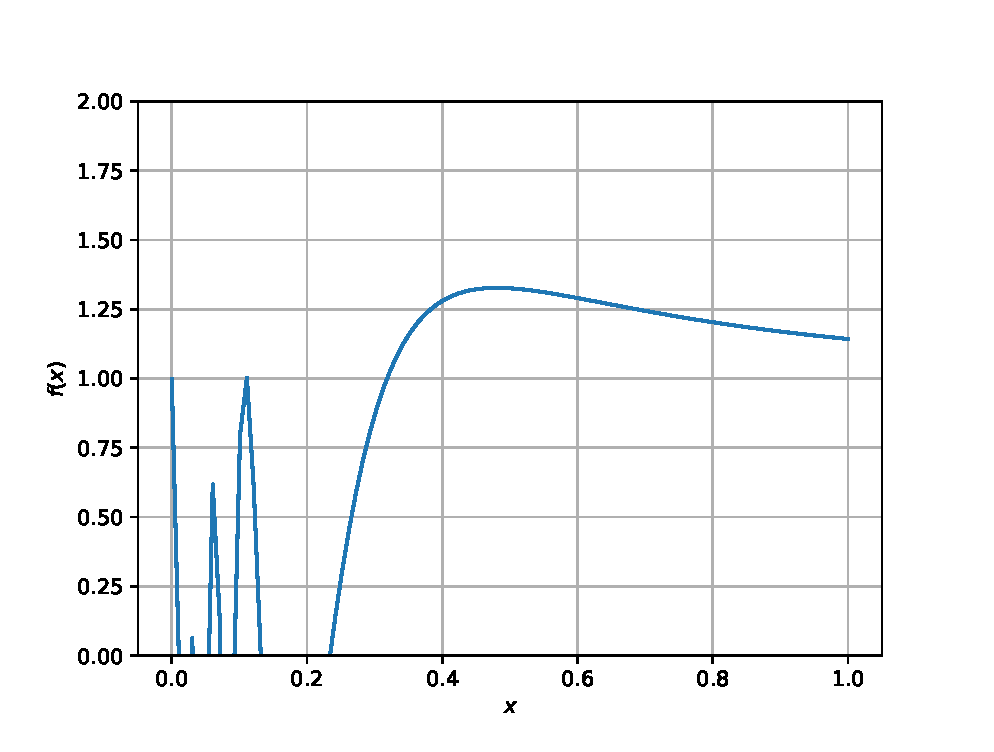
\includegraphics[width=\columnwidth]{./figs/2.eps}
%%\end{center}
%%\captionof{figure}{}
%%\label{fig:3}	
%%\end{figure}
%%
%%\begin{problem}
%%Show that the series defined by 
%%\begin{equation}
%%u_{n}=\sqrt{n+1}-\sqrt{n}
%%\end{equation}
%%diverges.
%%\end{problem}
%%\begin{proof}
%%Since
%%\begin{align}
%%S_n = \sum_{i=1}^{n}u_k = \sqrt{n+1}-1,
%%\end{align}
%%which is monotonically increasing as well as unbounded, $S_n$ diverges.
%%\end{proof}
%%%
%%\begin{proposition}
%%\label{prop:inequality}
%%Let the $n$th terms of two series be $a_n$ and $b_n$.  If $a_n < b_n$
%%\begin{enumerate}
%%\item  and the $b_n$ series converges, then the $a_n$ series also converges.
%%\item  and the $a_n$ series diverges, then the $b_n$ series diverges.
%%\end{enumerate}
%%\end{proposition}
%%\begin{problem}
%%\label{prob:inequality}
%%Sketch the series defined by 
%%\begin{equation}
%%u_{n}=\frac{2^n-1}{3^n}
%%\end{equation}
%%\end{problem}
%%%
%%\solution From Fig. \ref{fig:5}, it can be seen that the series converges.
%%%\input{./problems/ee16b1001.tex}
%%\lstinputlisting{./codes/5.py}
%%%
%%\begin{figure}[!ht]
%%\begin{center}
%%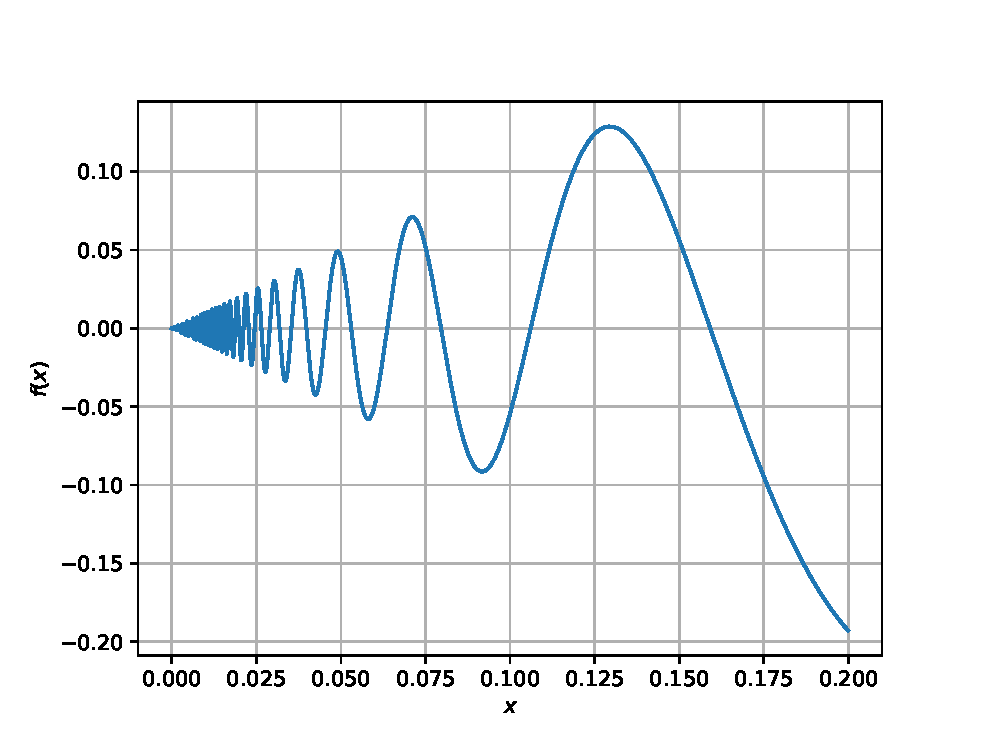
\includegraphics[width=\columnwidth]{./figs/5.eps}
%%\end{center}
%%\captionof{figure}{}
%%\label{fig:5}	
%%\end{figure}
%%
%%%
%%
%%\begin{problem}
%%Show that $S_n$ in Problem \ref{prob:inequality} converges.
%%\end{problem}
%%\solution Since
%%\begin{align}
%%u_{n}=\frac{2^n-1}{3^n} < \frac{2^n}{3^n},
%%\end{align}
%%using the root test, the $\frac{2^n}{3^n}$ series converges and from Proposition \ref{prop:inequality}, $S_n$ converges.
%%
%%\begin{proposition}
%%If $u_n$ is nonnegative and nonincreasing, then $S_n$ converges if and only if the $2^nu_{2^n}$ series converges.
%%\end{proposition}
%%\begin{problem}
%%Graphically examine the series 
%%\begin{equation}
%%u_{n}=\frac{1}{n\sqrt{n+1}}
%%\end{equation}
%%\end{problem}
%%\solution From Fig. \ref{fig:6}, it can be seen that the series converges.
%%%\input{./problems/ee16b1001.tex}
%%\lstinputlisting{./codes/6.py}
%%%
%%\begin{figure}[!ht]
%%\begin{center}
%%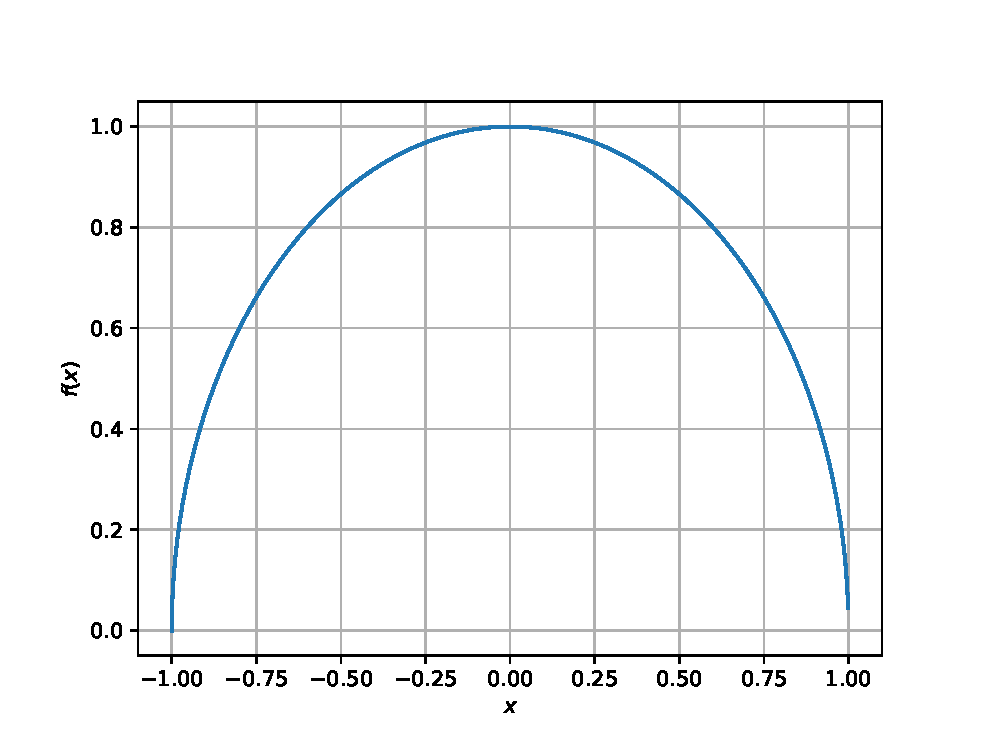
\includegraphics[width=\columnwidth]{./figs/6.eps}
%%\end{center}
%%\captionof{figure}{}
%%\label{fig:6}	
%%\end{figure}
%%
%%%
%%\begin{problem}
%%Show that 
%%\begin{equation}
%%u_{n}=\frac{1}{n\sqrt{n+1}}
%%\end{equation}
%%converges.
%%\end{problem}
%%\solution It is obvious that
%%\begin{equation}
%%u_n =\frac{1}{n\sqrt{n+1}} < \frac{1}{n\sqrt{n}} = f(n), \text{ say }
%%\end{equation}
%%Then,
%%\begin{align}
%%2^nf(2^n)&= \frac{2^n}{2^{\frac{3n}{2}}}
%%\\
%%&= \frac{1}{\brak{\sqrt{2}}^n}
%%\end{align}
%%which yields a convergent series using the root test. From Proposition \ref{prop:inequality}, it is obvious that $S_n$ converges.
%%\begin{proposition}
%%\label{prop:nonzero}
%%$S_n$ diverges if $\lim_{n\rightarrow \infty}u_n \ne 0$.
%%\end{proposition}
%%\begin{problem}
%%Graphically examine the series 
%%\begin{equation}
%%u_n = \frac{n}{n+1}
%%\end{equation}
%%\end{problem}
%%\solution From Fig. \ref{fig:4}, it can be seen that the series diverges.
%%%\input{./problems/ee16b1001.tex}
%%\lstinputlisting{./codes/4.py}
%%%
%%\begin{figure}[!ht]
%%\begin{center}
%%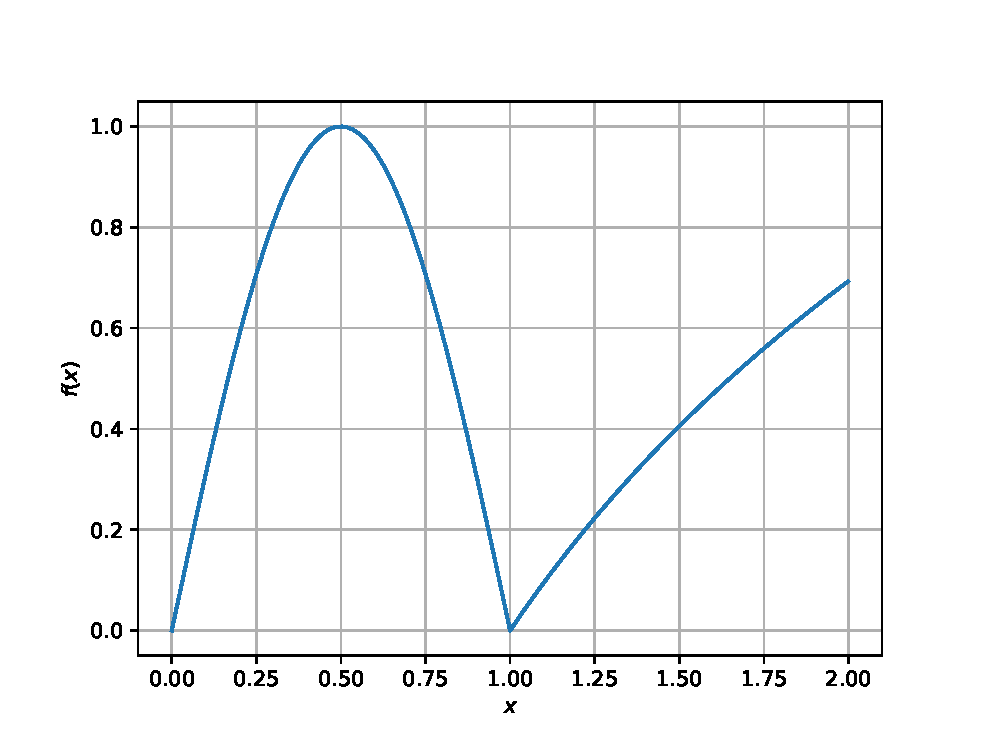
\includegraphics[width=\columnwidth]{./figs/4.eps}
%%\end{center}
%%\captionof{figure}{}
%%\label{fig:4}	
%%\end{figure}
%%
%%\begin{problem}
%%Show that 
%%\begin{equation}
%%u_n = \frac{n}{n+1}
%%\end{equation}
%%series diverges.
%%\end{problem}
%%\begin{proof}
%%Trivial using Propostion \ref{prop:nonzero}.
%%\end{proof}
%%\begin{proposition}
%%({\em Integral test}) Let $f(n)=u_n$ be positive and monotone decreasing. Then $S_n$ converges if
%%\begin{equation}
%%\lim_{t \rightarrow \infty}\int_{1}^{t}f(t)\, dt < \infty
%%\end{equation}
%%If the integral diverges, then $S_n$ also diverges.
%%\end{proposition}
%%%
%%\begin{problem}
%%Graphically examine the series 
%%\begin{equation}
%%u_n = \frac{1}{n}
%%\end{equation}
%%
%%\end{problem}
%%\solution From Fig. \ref{fig:2}, it can be seen that the series diverges.
%%%\input{./problems/ee16b1001.tex}
%%\begin{problem}
%%Show that 
%%\begin{equation}
%%u_n = \frac{1}{n}
%%\end{equation}
%%series diverges.
%%\end{problem}
%%\begin{proof}
%%Using the integral test,
%%\begin{align}
%%\lim_{t \rightarrow \infty}\int_{1}^{t}\frac{1}{t}\, dt = \lim_{t \infty}\ln t
%%\end{align}
%%which does not converge.  Hence the series diverges.
%%\end{proof}
%%\begin{proposition}
%%\label{prop:leibniz}
%%({\em Leibniz Test}) If
%%\begin{equation}
%%u_n = (-1)^na_n,
%%\end{equation}
%%then $S_n$ converges if
%%\begin{enumerate}
%%\item $a_n$ is monotonically decreasing
%%\item $\lim_{n\rightarrow \infty} a_n = 0$
%%\end{enumerate}
%%\end{proposition}
%%%
%%\begin{problem}
%%\label{prob:leibniz}
%%Graphically examine the series 
%%\begin{equation}
%%u_n = \frac{\cos n\pi}{\sqrt{n}}
%%\end{equation}
%%\end{problem}
%%\solution From Fig. \ref{fig:7}, it can be seen that the series converges.
%%%\input{./problems/ee16b1001.tex}
%%\lstinputlisting{./codes/7.py}
%%%
%%\begin{figure}[!ht]
%%\begin{center}
%%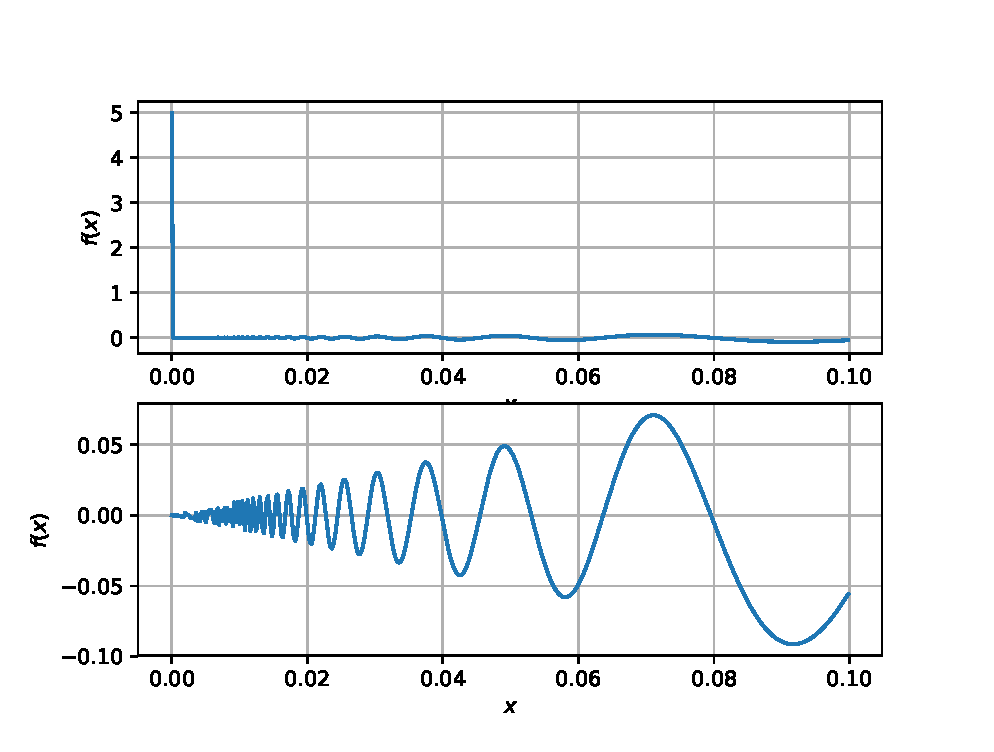
\includegraphics[width=\columnwidth]{./figs/7.eps}
%%\end{center}
%%\captionof{figure}{}
%%\label{fig:7}	
%%\end{figure}
%%
%%\begin{problem}
%%Show that 
%%\begin{equation}
%%u_n = \frac{\cos n\pi}{\sqrt{n}}
%%\end{equation}
%%converges.
%%\end{problem}
%%\begin{proof}
%%$\frac{1}{\sqrt{n}}$ is monotonically decreasing and goes to 0 as $n \rightarrow \infty$.  Using Proposition \ref{prop:leibniz}, $S_n$ converges.
%%\end{proof}
%%\begin{definition}
%%The series $\sum \limits _{{n=0}}^{m}\,u_{n}$ converges conditionally if $\lim \limits _{{m\rightarrow \infty }}\,\sum \limits _{{n=0}}^{m}\,u_{n} < \infty$  but
%%$\sum \limits _{{n=0}}^{\infty}\, \abs{u_n} = \infty$.
%%\end{definition}
%%\begin{problem}
%%Comment on the convergence of the series in Problem \ref{prob:leibniz}.
%%\end{problem}
%%\solution It was shown earlier that the
%%\begin{equation}
%%u_n = \frac{\cos n\pi}{\sqrt{n}}
%%\end{equation}
%%converges. 
%%For absolute convergence, it is necessary that
%%\begin{equation}
%%\abs{u_n} = \frac{1}{\sqrt n}
%%\end{equation}
%%series converge.  The following script generates Fig. \ref{fig:8}, indicating that the $\abs{u_n}$ series diverges.
%%\lstinputlisting{./codes/8.py}
%%%
%%\begin{figure}[!ht]
%%\begin{center}
%%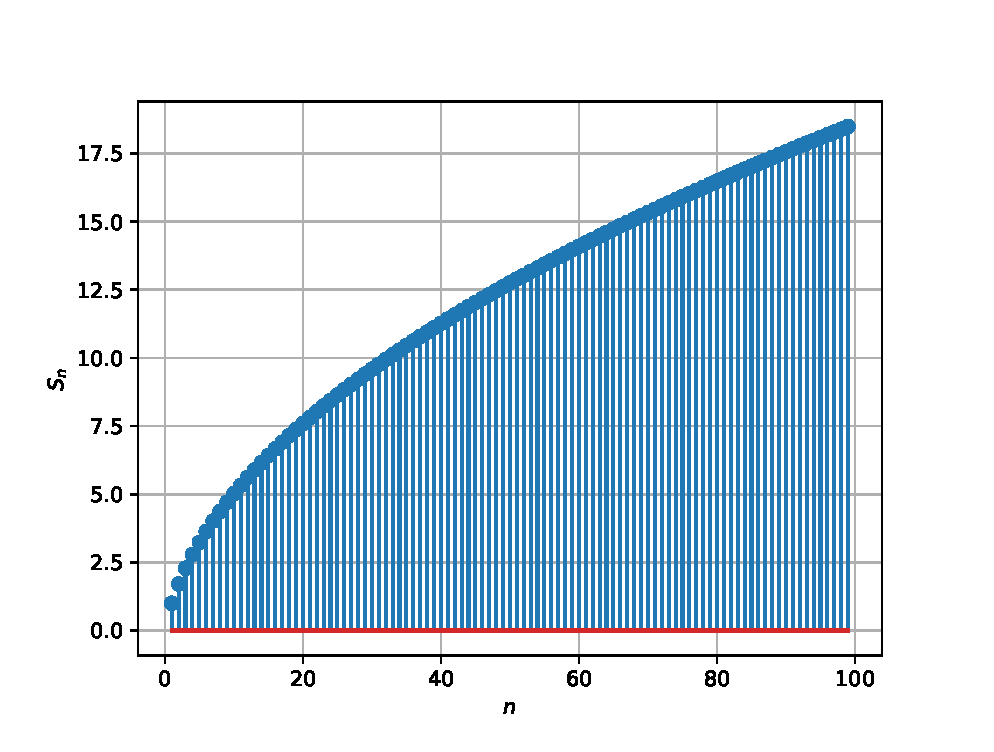
\includegraphics[width=\columnwidth]{./figs/8.eps}
%%\end{center}
%%\captionof{figure}{}
%%\label{fig:8}	
%%\end{figure}
%%Since
%%\begin{align}
%%\frac{1}{\sqrt{n}} > \frac{1}{n},
%%\end{align}
%%and $\sum \limits _{{n=1}}^{\infty}\,\frac{1}{n} $ diverges, from Proposition \ref{prop:inequality}, $\sum \limits _{{n=1}}^{\infty}\,\abs{u_n} $ diverges.  Hence $u_n$ 
%%is conditionally convergent.
\end{document}


